\chapter{Java Virtual Machine (JVM)}

This chapter focuses on the Java Virtual Machine (JVM). First the foundation and history of the JVM will be explained. Further focus is put on JVM itself and its functionality. In the following section the language of the JVM \textit{bytecode} is introduced. Finally, the bytecode manipulation tool ObjectWeb ASM is highlighted. This chapter is based on the specification of the JVM provided by \textcite{JVMHistoryOracle}.

\section{History}

 As the name suggests, the Java Virtual Machine is the virtual machine used to execute java programs. In 1994 Sun Microsystems Inc. developed the JVM because of their requirement for Java to be platform and operating system independent. By using a virtual machine as an intermediary, Sun was able to move the multiplatform aspect away from the compiler. 

One of the original use cases for Java and therefore the JVM was embedding of so-called applets in browsers. Applets were used in addition to the HTML document format, which at that time only provided limited functionality. Similar to HTML the applets were platform independent, which eased the development for the website creators. The first browser incorporating applets was HotJava. 

Java was originally closed source, however in 2006 Sun Microsystems Inc. began work on open sourcing the Java compiler and the JVM under the OpenJDK project \parencite{SunOpenSourceJava}. On November 13, 2006 the JVM implementation developed by Sun called HotSpot was open sourced under the GPL license.

The Version of the JVM specification is tied to the Java Version, but for the \texttt{class} files a separate version number so-called \textit{class file format version} is used. For the initial JDK release 1.0 the class file format version 45 was used. 

Various companies and organizations provide implementations of the JVM. For example GraalVM is an implementation of the JVM with the ability to perform ahead-of-time (AOT) compilation for a Java program. While this increases the performance of the application, it can only be executed on the platform it was compiled for. Another example is picoJava, which is a processor specification with the goal of enabling native execution of bytecode for embedded systems \parencite{PicoJava}. \textcite{PicoJavaFPGA} presented an implementation of picoJava on an FPGA.
%pico java

\section{Functionality}

The basic task of the JVM is to read a \texttt{class} file and execute the bytecode instructions contained in it. The specification defines only the abstract machine. How the bytecode is executed on the actual physical processor, or what optimizations are to be performed, is up to the implementer of the JVM specification. An official reference implementation of the JVM called OpenJDK\footnote{https://openjdk.org/} is provided by Oracle. 

\subsection{Architecture}

The JVM architecture can be seen in figure \ref{fig:JVMArchitecture}. It consists of the following elements: 

\begin{itemize}
    \item \textbf{Class Loader}: Loads \texttt{class} files into memory.
    \item \textbf{Runtime Data Area}: Manages all runtime memory used in the JVM.
    \item \textbf{Execution Engine}: Executes bytecode instructions.
    \item \textbf{Native Method Interface}: Interfaces with the native host system. 
\end{itemize}

\begin{figure}[]
    \centering
    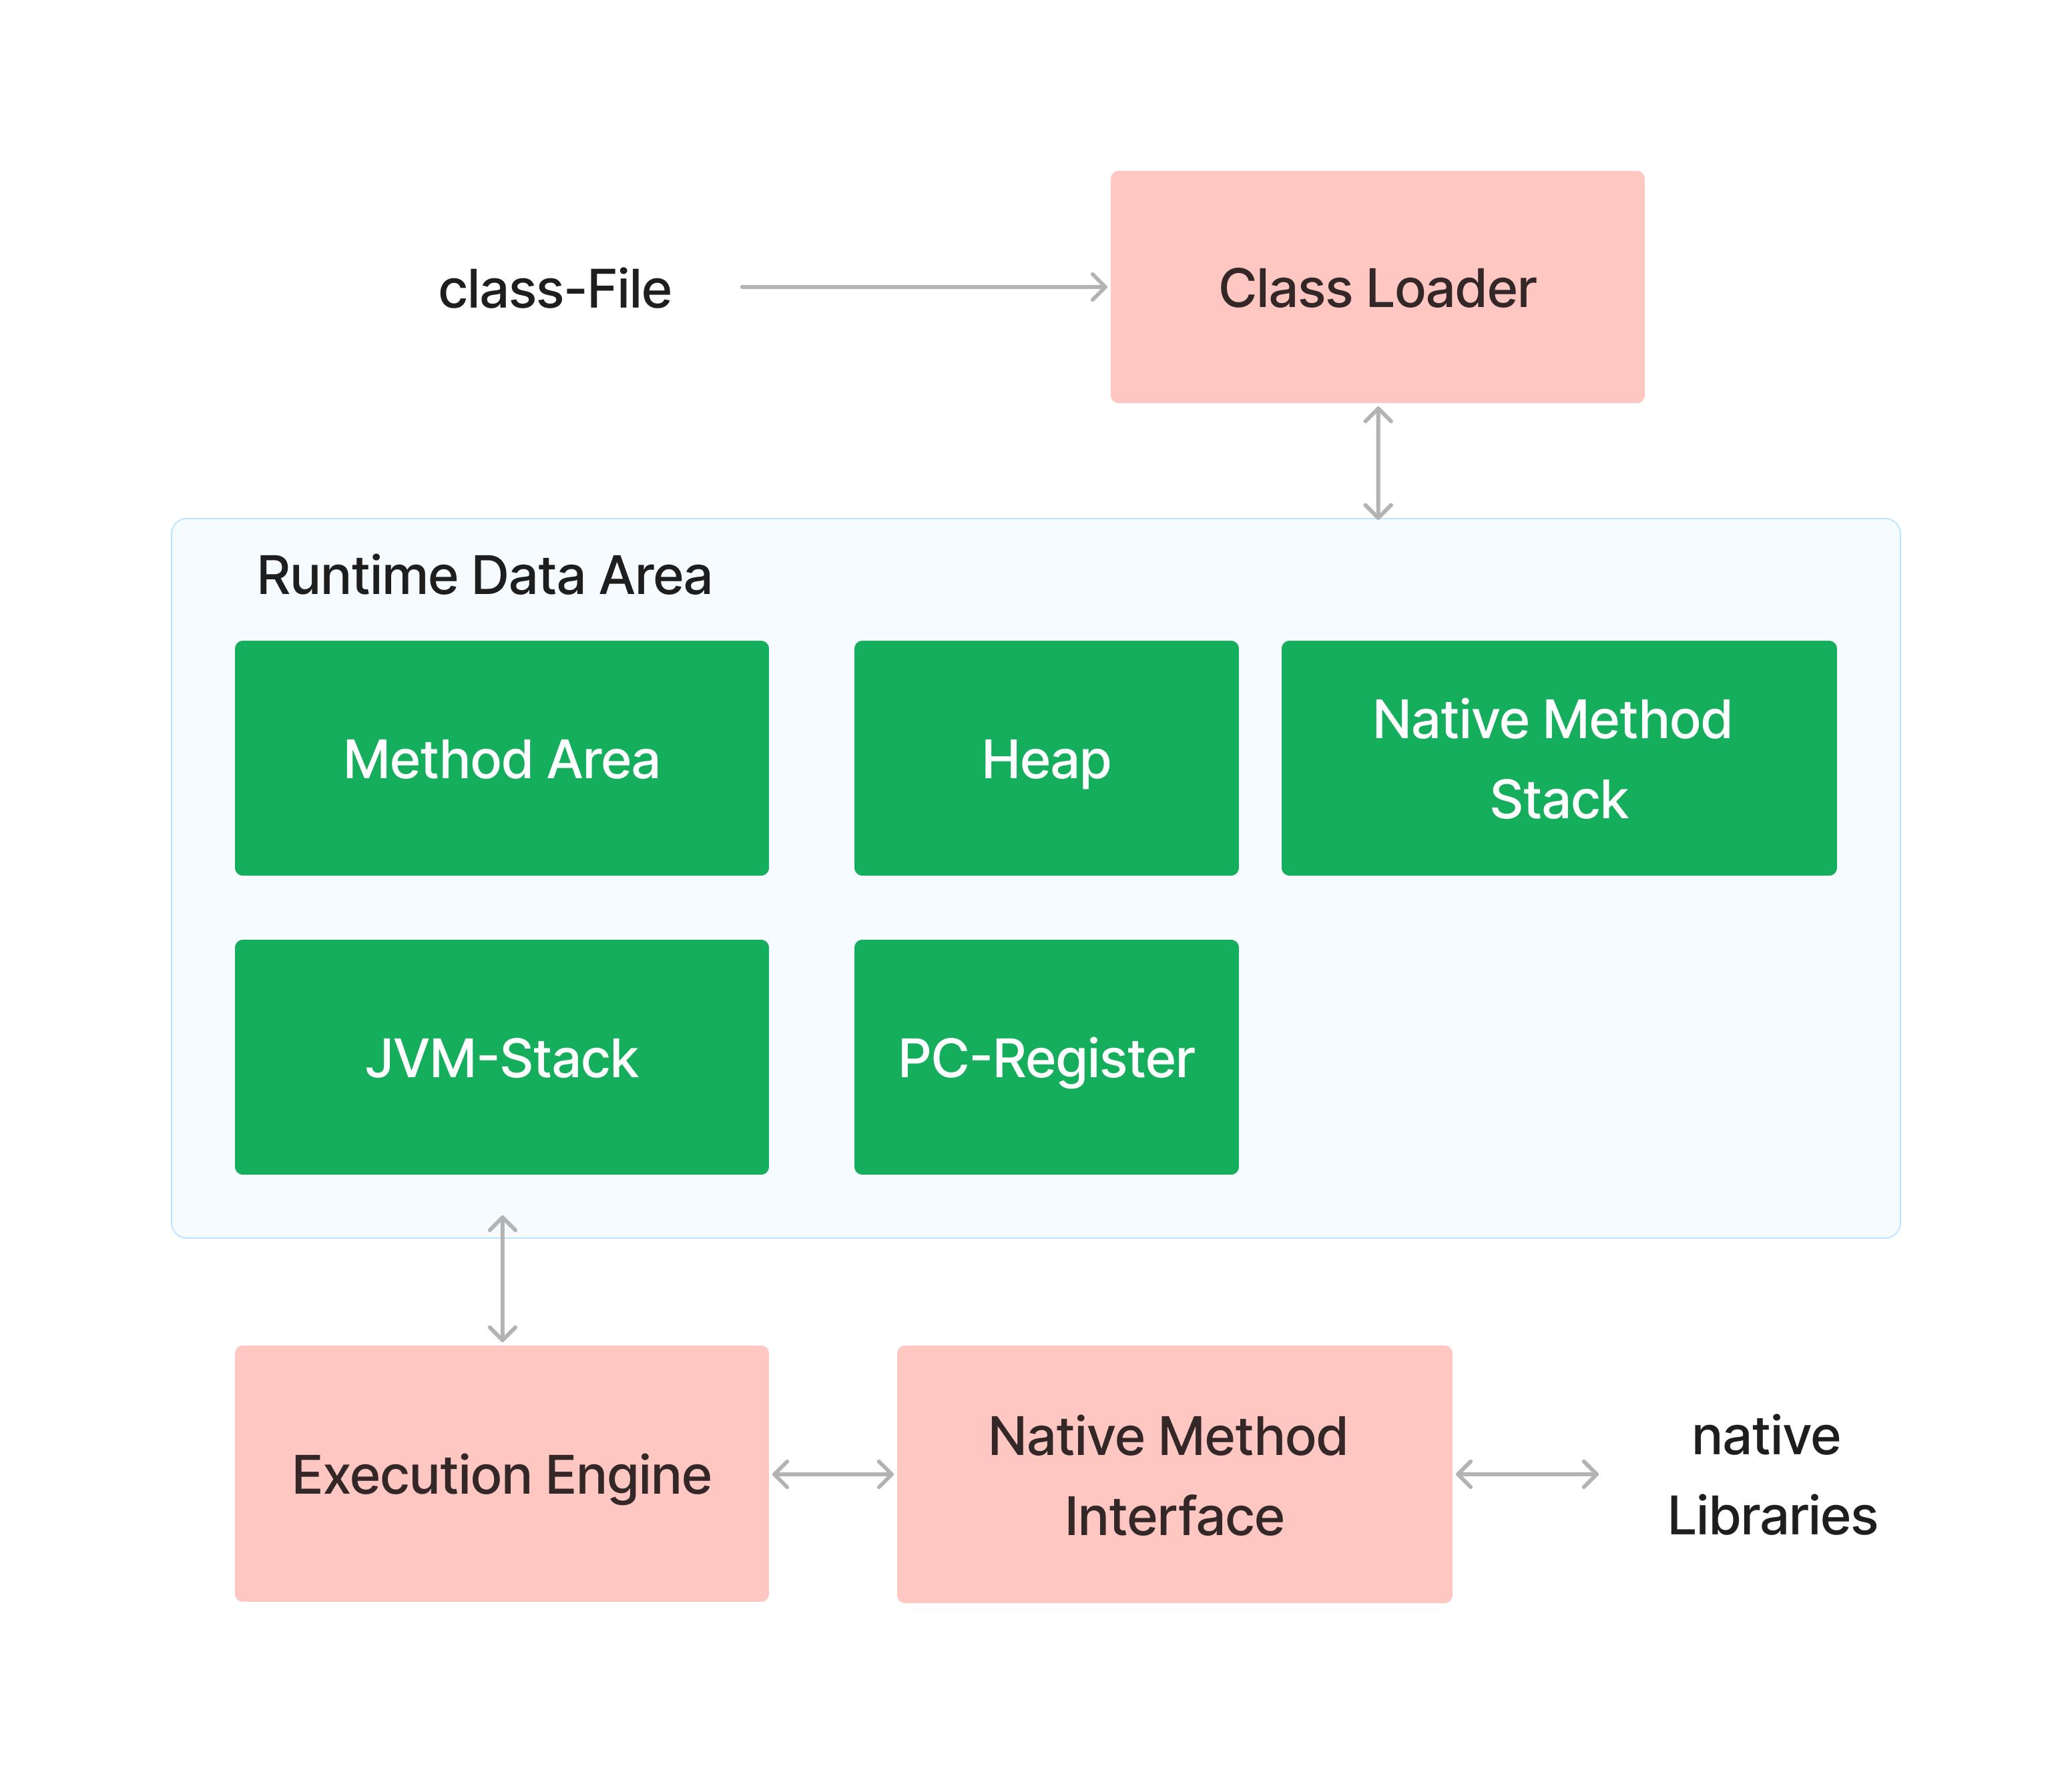
\includegraphics[width=\textwidth]{JVM_Architecture.png}
    \caption{Architecture of the JVM.}
    \label{fig:JVMArchitecture}
\end{figure}

\subsubsection{Class Loader}

The class loader takes care of loading bytecode into the JVM memory. There are three tiers of class loaders:

\begin{itemize}
    \item \textbf{Bootstrap}: Loads JDK internal classes and core libraries. Implemented in native code and not accessible by an application. 
    \item \textbf{Extension}: Loads extensions of the standard Java classes from the JDK extensions directory. 
    \item \textbf{Application}: Loads all application level classes. These are located via the classpath. Classes can be put on the classpath by using an environment variable or command line option. 
\end{itemize}

The class loaders are organized in a parent-child hierarchy. The Bootstrap class loader is the parent of the Extension class loader, which itself is the parent of the Application class loader. When a request is made to load a \texttt{class} file, the class loader first delegates the request to its parent class loader. Only if the parent class loader cannot locate the class the current class loader will attempt to load it. This process is performed so that no two class loaders attempt to load the same class. The loading process is separated into three stages. Loading, linking and initialization.

In the loading stage the bytecode is loaded into the JVM. The bytecode can be loaded from a file, the network or another source. The bytecode is loaded into the JVM as a \texttt{Class} object.

In the second stage linking is performed. This stage is separated into the three substages verification, preparation and resolution. Verification is performed to ensure that the loaded bytecode adheres to the JVM's rules. Rules include such as requiring that a return instruction must match its method's return type, or that a \texttt{throw} instruction must only throw values that are instances or subclasses of \texttt{Throwable}. Verification is performed because the JVM must guarantee that only correct \texttt{class} files are executed and no exploitation through malicious bytecode is taking place. The second substage preparation creates the static fields of a class or interface and allocates the memory needed for them. The static fields further are assigned their respective default values. Explicit initializers are executed during initialization, during preparation no bytecode is executed. Resolution then resolves all symbolic references inside the class. Symbolic references are used for example when referencing another class or interface. For each symbolic reference resolution determines a concrete value. 

If linking has been successful the class or interface is initialized. Explicit initializer of static fields are executed as are static initializer blocks of the class or interface.



%The JVM specification describes the structure and functionality of the JVM in the following areas:



%\begin{itemize}
%    \item \texttt{class} File Format
%    \item Data Types
%    \item Runtime Data Areas
%    \item Method Frames
%    \item Arithmetic Operations
%    \item Special Methods
%    \item Exceptions
%    \item Instruction Set
%    \item Support for Class Library
%\end{itemize}







%The JVM only understands bytecode, but not Java source code. Other programming languages also target the JVM for execution. For example the programming   

%first third party ibm j9

%Instead of compiling a Java program to native machine code for a specific operating system and platform, the Java compiler produces so called \textit{bytecode} in the binary \texttt{class} file format. The JVM reads the class file and the instructions included in it. The bytecode instructions are then processed by the JVM and appropriate machine code is executed.  
